\chapter{Lua Environment} \label{lua}

Currently, the web browser cannot execute the Lua code, as the Lua environment is not readily available in the browser. In this project, we will use the Lua VM provided by Mozilla \cite{luavm} to provide Lua support for the browser. The Lua VM will create Lua environment where we will be able to execute our program written in Lua.

\section{The Lua VM}

The Lua VM runs in the browser by porting the entire ANSI C implementation of the Lua virtual machine to JavaScript using Emscripten \cite{emscripten} including garbage collection.

The Lua VM can be added in the web page by referencing ``lua.vm.js'' script on the browser, as shown below.

\begin{lstlisting}
    <script src=``lua.vm.js''></script>
\end{lstlisting}

Once the instance of the Lua VM is added on the web page, we can start writing our Lua code in the web page by including all the Lua code in the text/lua script as shown Figure \ref{fig:luascript}.

\begin{figure}[h]
	\begin{lstlisting}
	<script type=``text/lua''>
	...your lua code
	</script>
	\end{lstlisting}
	\caption{Lua script example}
	\label{fig:luascript}
\end{figure}

The Lua VM interpretes the code written in ``$<$script type="text/lua" $>$ $<$/script$>$" tags, and it executes it as Lua code.

\subsection{Examples}

In this section, we will see some of the examples using the Lua VM in the browser.

\textbf{1. Showing alert on the web page using Lua}

Example shown in Figure \ref{fig:luaalertcode} renders alert method of JavaScript global object using Lua.  

\begin{figure}[h]
	\begin{lstlisting}
	<script src=``lua.vm.js''></script>
	
	<script type=``text/lua''>
	 js.global:alert(`hello from Lua script tag in HTML!')
	</script>
	\end{lstlisting}
	\caption{Showing alert on the web page using Lua}
	\label{fig:luaalertcode}
\end{figure}


Executing the code from Figure \ref{fig:luaalertcode} in the browser generates output similar to calling alert function from DOM, as shown in Figure \ref{fig:luaalert}.

\begin{figure}[H]
	\begin{center}
		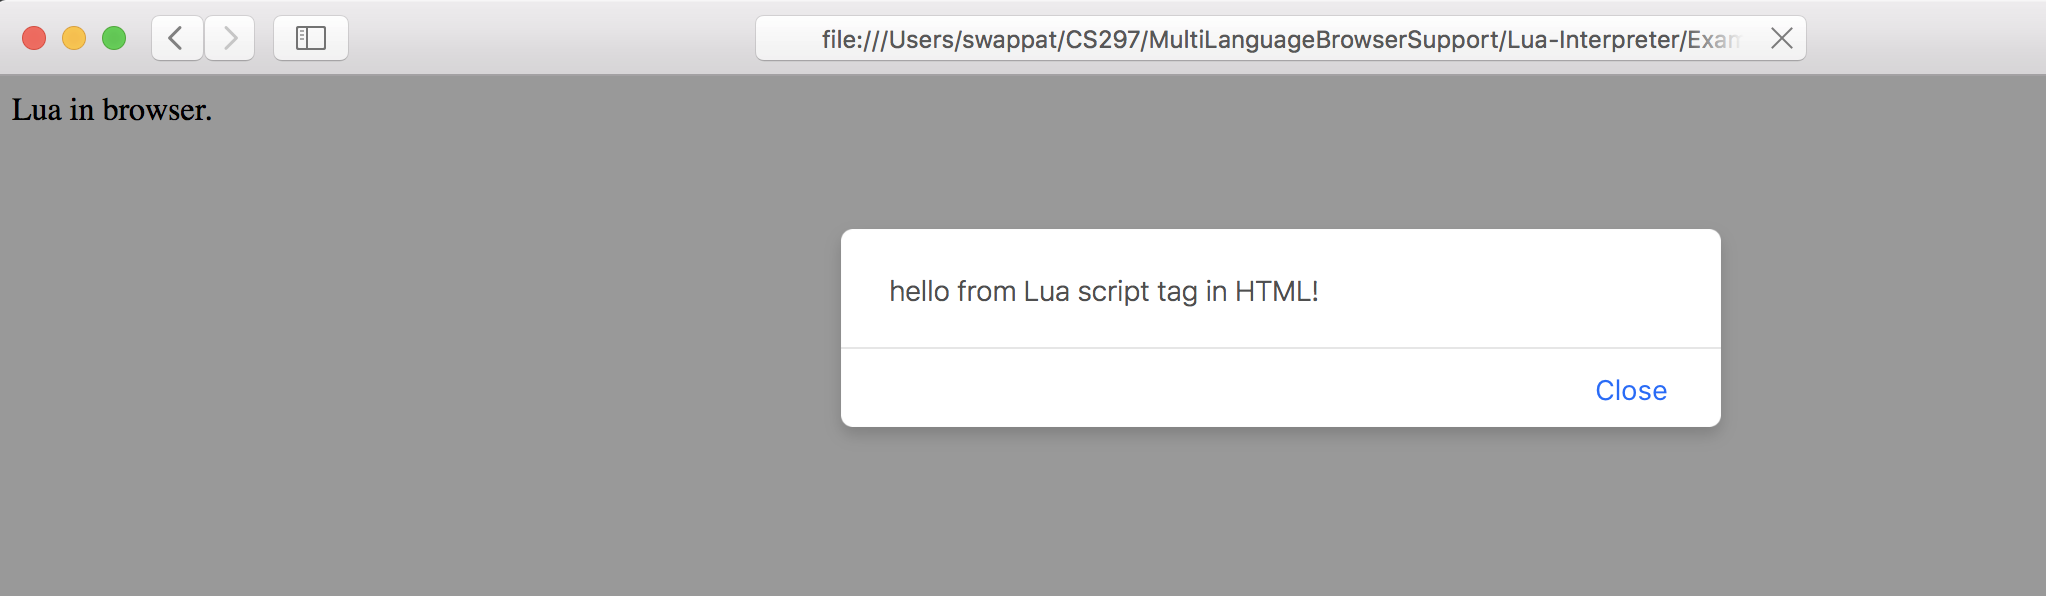
\includegraphics[width=\linewidth]{./images/lua-alert.png}
	\end{center}
	\caption{Showing alert on the web page using Lua: Output}
	\label{fig:luaalert}
\end{figure}

\textbf{2. Executing a Lua function in the browser}

We can also define and call a Lua function in the web page, as shown in Figure \ref{fig:luafunctioncode}.

\begin{figure}[h]
	\begin{lstlisting} 	
	<script src=``lua.vm.js''></script>
	<script type=``text/lua''>
	-- function
	function printName (recipient)
	print(`Hello, '..recipient)
	end
	-- Anonymus function
	local sayHello = function (recipient)
	print(`Hello, '..recipient)
	end
	sayHello(`Swapnil')
	printName(`CS298 Project')
	</script>
	\end{lstlisting}
	\caption{Executing a Lua function in the browser}
	\label{fig:luafunctioncode}
\end{figure}


Executing the code from Figure \ref{fig:luafunctioncode} in the browser creates a function called ``printName" and assigns anonymous function to the local variable named ``sayHello". After calling both functions, we see the desired output on the console, as shown in Figure \ref{fig:luafunction}.

\begin{figure}[H]
	\begin{center}
		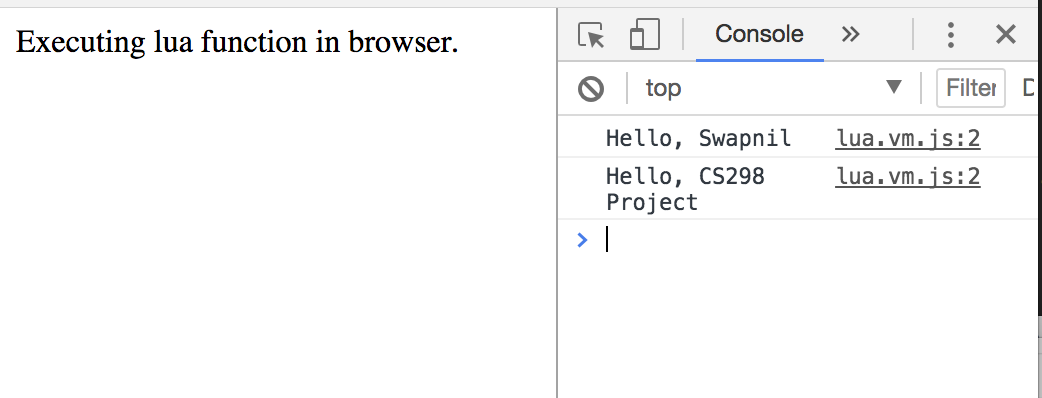
\includegraphics[width=\linewidth]{./images/lua-functions.png}
	\end{center}
	\caption{Executing Lua function in the browser: Output}
	\label{fig:luafunction}
\end{figure}


\section{Approach}

Similar to the Scheme environment, we implemented browser plugin approach to include Lua VM in the web page, to help browser understand Lua code on the web page.

For this approach, browser plugin (supported by Firefox and Chrome) will push the instance of Lua VM in every newly opened browser tab. In this way, user doesn't have to worry about adding the library script on the page. Lua VM library will then interpret all the code enclosed within ``type=text/lua" script.

In case of using a browser plugin, our example code to render alert in the browser is shown in Figure \ref{fig:luaalertplugin}.

\begin{figure}[H]
	\begin{lstlisting}
	<script type=``text/lua''>
	js.global:alert(`hello from Lua script tag in HTML!') 
	</script>
	\end{lstlisting}
	\caption{Lua alert with browser plugin}
	\label{fig:luaalertplugin}
\end{figure}

As shown in the code snippet from Figure \ref{fig:luaalertplugin}, we don't need to add any external libraries in our webpage to interpret Lua script, browser plugin will take care of it.
Executing above code in the browser with our plugin installed will alert the user with ``hello from Lua script tag in HTML!" as text.


\subsection{JS Library}

Whenever plugin is unavailable the Lua VM support is achieved in the web page by including the Lua VM library in the web page itself. When the web page is loaded in the browser, our library will read code snippet inside ``type=text/lua" script and will interpret it, as shown in Figure \ref{fig:luaalertcode}.